% ****** Start of file apssamp.tex ******
%
%   This file is part of the APS files in the REVTeX 4.1 distribution.
%   Version 4.1r of REVTeX, August 2010
%
%   Copyright (c) 2009, 2010 The American Physical Society.
%
%   See the REVTeX 4 README file for restrictions and more information.
%
% TeX'ing this file requires that you have AMS-LaTeX 2.0 installed
% as well as the rest of the prerequisites for REVTeX 4.1
%
% See the REVTeX 4 README file
% It also requires running BibTeX. The commands are as follows:
%
%  1)  latex apssamp.tex
%  2)  bibtex apssamp
%  3)  latex apssamp.tex
%  4)  latex apssamp.tex
%
\documentclass[%
 reprint,
%superscriptaddress,
%groupedaddress,
%unsortedaddress,
%runinaddress,
%frontmatterverbose, 
%preprint,
%showpacs,preprintnumbers,
%nofootinbib,
%nobibnotes,
%bibnotes,
 amsmath,amssymb,
 aps,
%pra,
%prb,
%rmp,
%prstab,
%prstper,
%floatfix,
]{revtex4-1}

\usepackage{graphicx}% Include figure files
\usepackage{dcolumn}% Align table columns on decimal point
\usepackage[spanish]{babel}
\selectlanguage{spanish} 
\usepackage[utf8]{inputenc}
\usepackage{bm}% bold math
%\usepackage{hyperref}% add hypertext capabilities
%\usepackage[mathlines]{lineno}% Enable numbering of text and display math
%\linenumbers\relax % Commence numbering lines
\usepackage{float}
%\usepackage[showframe,%Uncomment any one of the following lines to test 
%%scale=0.7, marginratio={1:1, 2:3}, ignoreall,% default settings
%%text={7in,10in},centering,
%%margin=1.5in,
%%total={6.5in,8.75in}, top=1.2in, left=0.9in, includefoot,
%%height=10in,a5paper,hmargin={3cm,0.8in},
%]{geometry}

\usepackage{hyperref} 
\begin{document}

%\preprint{APS/123-QED}

\title{Espectros Atómicos}% Force line breaks with \\

\author{Maria Laura Pérez Lara}
\email{ml.perez11@uniandes.edu.co}
 \altaffiliation[Also at ]{Departamento de Física, Universidad de los Andes}
\author{Julián Rodríguez Cardona}%
 \email{jl.rodriguez11@uniandes.edu.co}
\affiliation{Departamento de Física, Universidad de los Andes}%

%\collaboration{}%\noaffiliation

\date{\today}% It is always \today, today,
             %  but any date may be explicitly specified

\begin{abstract}
El presente experimento se realiza con dos fines: Observar las líneas de emisión de varios elementos usando un prisma y una rejilla de difracción; y relacionar una longitud de onda conocida de las líneas espectrales con una variable de longitud, para luego extrapolar la relación y medir cuantitativamente un espectro que en principio es desconocido. Para ello, se utiliza un espectrómetro que consta de un colimador, un telescopio, una regla amplificada mediante una lámpara auxiliar y el prisma. Al poner diversas lámparas de gases de elementos frente al colimador, su luz experimenta el fenómeno de difracción que podrá ser captada por el telescopio, y las líneas espectrales se observan en lugares específicos de la escala longitudinal. Tomando como calibración la lámpara de Mercurio y sus líneas espectrales de valores de $\lambda$ conocidos, se obtuvo una relación entre la variable longitudinal y dichos valores de $\lambda$ dada por $\lambda = -19.94X+755.336$, que fue utilizada para calcular las longitudes de onda de líneas espectrales en He, H, Hg, Xe, Kr, Ne y Ar, donde para los dos primeros elementos, el error medio fue de 11.8\%. En particular, para el H se calculó la constante de Rydberg con los valores hallados y las transiciones conocidas de niveles energéticos, de manera que el valor más cercano le correspondió, con un error de 2.3\%, a la transición de la línea roja $(n: 3 \rightarrow 2)$ con $R_H= 10720858.62 m^{-1}$. 

\end{abstract}

\maketitle

%\tableofcontents

%---------------------INTRODUCCIÓN------------------
\section{Introducción}

A prinicipios del siglo XIX, Niels Bohr propuso un modelo atómico en donde los electrones giran alrededor de su núcleo en ciertas órbitas permitidas de carácter circular, con un momento angular cuantizado. Esta teoría sugiere que dichos electrones tienen ciertos niveles de energía determinados, para lo cual es posible analizar lo que ocurre al excitarlos. Por la conservación de energía, al llevar a un electrón a un estado excitado de energía y que este se regrese a su estado base, se debe entonces liberar un fotón que tenga exactamente la misma energía que la diferencia de energías del electrón, lo cual implica que la longitud de onda $\lambda$ del fotón liberado dependa de estos "saltos'' energéticos que realizan los electrones. Dependiendo de la identidad del átomo, las transiciones que se llevan acabo son distintas y por ende, cada átomo es capaz de emitir un set específico de líneas espectrales que son observadas y diferenciadas gracias al fenómeno de difracción de la luz total emitida. \\
La excitación se puede lograr al someter a un gas de átomos del mismo tipo a una diferencia de potencial (como en las lámparas de gases), los cuales emiten luz que, al pasar por un elemento difractivo, se descompondrá en líneas que evidencian las longitudes de onda correspondientes a los saltos energéticos permitidos. Este fenómeno es fundamental para evidenciar la teoría cuántica atómica gracias a la nitidez de las líneas de emisión espectrales, aunque esta nitidez y exactitud en su localización puede verse afectada por factores como lo son el efecto Doppler (los átomos se mueven con respecto al observador, por lo cual podría haber un shifting hacia el rojo si se aleja o el azul si se acerca), el desdoblamiento de los niveles (gracias al efecto Zeeman en presencia de campo magnético externo o el efecto Stark en presencia de campo eléctrico externo) y la existencia de un ancho en las líneas debido a los dos elementos anteriores, aunque este ancho no debería tener un error significativo en espectroscopía. \cite{width}\\
Para obtener una relación entre la longitud de onda y los niveles energéticos involucrados, se utiliza la fórmula de Balmer, la cual surge de las suposiciones del modelo atómico de Bohr y conceptos de mecánica clásica. Considere un átomo de hidrógeno con el protón inmóvil en el origen. La fuerza de Coulomb entre el electrón y el protón será la fuerza que genere aceleración centrípeta. A partir de esta relación en conjunto con la segunda ley de Newton, se obtiene la velocidad del electrón:

\begin{equation}
    Fc=\frac{e^2}{4\pi\epsilon_0 r^2}=\frac{m_ev^2}{r}\rightarrow v=\sqrt{\frac{e^2}{4\pi \epsilon_0 rm_e}}.
    \label{eq:velocidad}
\end{equation}

Si el momento angular del electrón es $L=m_evr$ y está cuantizado ($L=n\hbar$), es posible hallar una expresión para el radio atómico a partir de lo anterior y la ecuación \ref{eq:velocidad}, de manera que el radio también estará cuantizado:

\begin{equation}
    r=\frac{n^2\hbar^2 4\pi\epsilon_0}{m_ee^2}.
    \label{eq:radio}
\end{equation}

En adición, si se hace un análisis con la energía, se tiene que el electrón posee energía cinética clásica $p_e^2/2m_e$ y un potencial $-e^2/4\pi\epsilon_0r$. Si el momento lineal también está cuantizado ($p_e=n\hbar/r$), podemos hallar que, con el radio de la ecuación \ref{eq:radio}, la energía está cuantizada también:

\begin{equation}
    E_n=\frac{-m_ee^4}{2\hbar^2(4\pi\epsilon_0)^2}\frac{1}{n^2}.
    \label{eq:energiaH}
\end{equation}

Ahora bien, la energía del fotón liberado debe de ser igual a la diferencia de las energías, de manera que $E_f=\frac{hc}{\lambda}=E_{n_1}-E_{n_2}$ con $n_1 < n_2$. Uniendo esto a la ecuación \ref{eq:energiaH}, se obtiene la \textbf{fórmula de Balmer}:

\begin{equation}
    \frac{1}{\lambda}=\frac{m_ee^4}{8h^3c\epsilon_0^2}(\frac{1}{n_1^2}-\frac{1}{n_2^2}).
    \label{eq:Balmer}
\end{equation}

Entonces se define la \textbf{constante de Rydberg} como la constante que acompaña el término de diferencia entre niveles:

\begin{equation}
    R_H=\frac{m_ee^4}{8h^3c\epsilon_0^2}=10973731.568508 m^{-1}.
    \label{eq:Rydberg}
\end{equation}

Para comparar los valores de longitudes de onda experimentales, se tienen los siguientes valores teóricos (algunas transiciones no pudieron ser halladas):

\begin{table}[H]
    \centering
    \begin{tabular}{|c|c|c|c|}
    \hline
    Elemento & $\lambda (nm)$ & Color & Transición \\ \hline
    Hidrógeno & 434.1 & Violeta & $5\rightarrow2$ \\
     & 486.1 & Azul & $4D\rightarrow2P$ \\
     & 656.3 & Rojo & $3D\rightarrow2P$ \\ \hline
    Helio & 447.148 & Violeta & $4^3D\rightarrow2^3P$ \\
     & 471.314 & Azul & $4^3S\rightarrow2^3P$ \\
     & 492.193 & Cian & $4^1D\rightarrow2^1P$ \\
     & 501.567 & Amarillo & $3^1P\rightarrow2^1S$\\
     & 587.56 & Rojo & $3^3D\rightarrow2^3P$\\
     & 667.815 & Rojo & $3^1D\rightarrow2^1P$\\ \hline
    Mercurio & 435.83 & Azul & $3P\rightarrow3S$ \\
     & 546.07 & Verde & $3P\rightarrow3S$ \\
     & 576.96 & Amarillo & - \\
     & 579.07 & Amarillo & - \\ \hline
    \end{tabular}
    \caption{Valores teóricos de los espectros de H, He y Hg.\cite{nist}}
    \label{tab:teoria}
\end{table}

Finalmente y para mejor visualización, los espectros del Kriptón, Xenón, Argón, Neón tienen el siguiente aspecto (cuantitativamente se usarán comparaciones con los datos de longitudes de onda \cite{nobles}): 

\begin{figure}[H]
    \centering
    \includegraphics[scale=0.27]{espectros_nobles.png}
    \caption{Espectros de emisión de Ne, Ar, Kr y Xe. \cite{ohio}}
    \label{fig:espectrosnobles}
\end{figure}
%----------------------MONTAJE----------------


\section{Montaje Experimental y Metodología}
El montaje consta de un espectrómetro, un prisma, una rejilla de difracción (se utiliza aparte, solo para comparar lo visto con el prisma), una lámpara de descarga y tubos de gases de H, He, Hg, Kr, Ar, Xe y Ne. El espectrómetro en sí consta de un colimador, un telescopio y una lámpara auxiliar con una regla incorporada, para que al poner el prisma en el centro y observar la difracción de la luz del tubo en la lámpara de descarga, las líneas espectrales se observen junto con la escala longitudinal. Este montaje se observa en la siguiente imagen:

\begin{figure}[H]
    \centering
    \includegraphics[scale=0.7]{montaje_espectros.png}
    \caption{Montaje experimental. Se observa el espectrómetro y el colimador apuntando a la lámpara de descarga. \cite{guia}}
    \label{fig:montaje}
\end{figure}

La metodología consiste primero en tomar el tubo de Hg, ponerlo en la lámpara de descarga frente al colimador (con su rejilla previamente ajustada) y observar, en un ambiente de mínima luz, su espectro en el telescopio, teniendo en cuenta de ir girándolo (en sentido antihorario) junto con el prisma hasta lograr observar las líneas espectrales y la regla en la misma imagen y en lo posible a la misma altura para mayor precisión en la medida longitudinal de cada línea conocida del espectro. Con esto, se comparan las líneas teóricas (con ayuda de lo visto en la rejilla de difracción para observar los colores) y se realiza la relación lineal entre el parámetro longitudinal medido y la longitud de onda teórica mediante una regresión lineal de los datos de varias líneas conocidas, para que posteriormente cada medida de los demás espectros pueda convertirse a un valor de $\lambda$.\\
Después de hacer la calibración, se observan de la misma manera los espectros de H y He, midiendo los parámetros longitudinales y calculando sus longitudes de onda con la relación hallada. En particular, para el H, se calcula la constante de Rydberg sabiendo la información del cuadro \ref{tab:teoria} y haciendo uso de la ecuación \ref{eq:Balmer}.\\
Finalmente, se hace el análisis con los tubos de los gases restantes, y se miden sus líneas espectrales con mayor intensidad, y se compara tanto con el espectro general mostrado en la figura \ref{fig:espectrosnobles}, como con los valores de todas sus longitudes de onda permitidas. \cite{nobles}

%-----------------RESULTADOS----------------------
\section{Resultados y Análisis}

\subsection{Calibración del espectrómetro}

Primero, se tuvo que realizar la calibración del espectrómetro utilizado en la práctica. Para esto, se ubicó el montaje y se observó el espectro del átomo de mercurio (Hg), de manera que se observara el espectro de éste en el rango de la regleta del espectrómetro. De esta forma, se tomaron datos de las longitudes de onda de las líneas espectrales en las unidades arbitrarias de la regla del instrumento, se compararon con las teóricas y se obtuvo una relación entre estas dos unidades de medición. Estos se consignaron en la siguiente tabla.

\begin{table}[H]
    \centering
    \begin{tabular}{|c|c|c|}
    \hline
    Color & $\lambda$ (Escala espectrómetro) & $\lambda_{teórica}$ (nm) \\ \hline
    Amarillo 2 & 8.7 & 579.07 \\ \hline
    Amarillo 1 & 8.8 & 576.96 \\ \hline
    Verde & 10.9 & 546.07 \\ \hline
    Azul & 15.9 & 435.83 \\ \hline
    \end{tabular}
    \caption{Medidas de longitud de onda de lineas espectrales del Mercurio (Hg). Los datos teóricos fueron tomados de \cite{nist}}
    \label{tab:calibracion}
\end{table}

A partir de los datos anteriores, se pudo obtener una regresión lineal que nos brindara una equivalencia entre la escala arbitraria de la regleta del espectrómetro y la medida en nanómetros para la longitud de onda de las lineas espectrales. La regresión lineal extraída de los datos fue la siguiente:

\begin{equation}
 \lambda = -19.94 X + 755.336
\end{equation}

Donde $X$ se refiere a la medida en la escala arbitraria del instrumento y $\lambda$ a la medida en nanómetros, ambas medidas para las longitudes de onda de las líneas espectrales que se observan.

Los datos y la regresión realizada se presentan en la siguiente gráfica.

\begin{figure}[H]
    \centering
    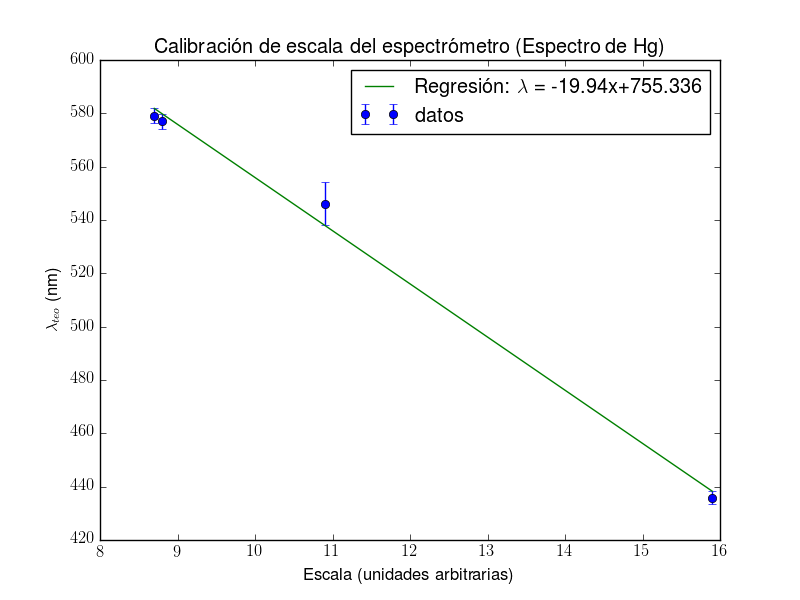
\includegraphics[scale=0.4]{calibracion.png}
    \caption{Regresión lineal de la calibración del espectrómetro utilizando las lineas espectrales del Mercurio.}
    \label{fig:calibracion}
\end{figure}

Así pues, el ajuste realizado se utilizó para determinar valores en unidades conocidas (nm) de las mediciones de longitud de onda que se mostrarán en las siguientes actividades del experimento en cuestión. Además, se determinó que si la abertura que posee el colimador se ensancha, también lo hacen las líneas y a la vez aumenta la intensidad de éstas; de manera análoga, si se angosta la abertura, las líneas espectrales también se angostan y a la vez se reduce su intensidad.

Asimismo, se observaba que ciertas líneas espectrales eran más intensidad que otras, lo cual se debe precisamente a que la intensidad de éstas depende de la probabilidad de transición entre dos estados, lo cual se conoce como las reglas de selección, y también a la tasa de emisión neta. \cite{intensidad}

\subsection{Líneas espectrales de H, He y constante de Rydberg}

Teniendo el ajuste de la primera actividad, se procedió a realizar las mediciones de longitud de onda de las líneas espectrales de los elementos Hidrógeno (H) y Helio (He). Los datos obtenidos están consignados en la siguiente tabla:

\begin{table}[H]
    \centering
    \begin{tabular}{|c|c|c|c|c|}
    \hline
    Elemento & Color &  $\lambda$ ( $\pm 0.1$ ua) & $\lambda$ ($\pm$ 6.68 nm) & \% error \\ \hline
    Hidrógeno & Rojo  & 4.2 & 671.588 & 2.33 \\ 
     & Azul & 16.4 & 428.32 & 11.89 \\ 
     & Violeta &  19.4 & 368.5 & 15.11 \\ \hline
    Helio & Rojo 2  & 3.7 & 681.558 & 2.06 \\ 
     & Rojo 1 & 5 & 655.64 & 11.58\\ 
     & Amarillo  & 8.1 & 593.82 & 18.4 \\ 
     & Azul claro & 14.8 & 460.224 & 6.49 \\ 
     & Azul oscuro & 15.8 & 440.284 & 6.58 \\ 
     & Violeta & 22.5 & 306.686 & 31.41 \\ \hline
    \end{tabular}
    \caption{Medidas de longitud de onda de líneas espectrales del \textbf{Hidrógeno} (H) y el \textbf{Helio} (He) . El error se hace respecto a los datos teóricos presentados en \ref{tab:teoria}. Se aclara que ''ua" se refiere a las unidades arbitrarias de la escala del espectrómetro.}
    \label{tab:nobles}
\end{table}

Para el Helio, observamos que, en general, los porcentajes de error son modestos, exceptuando el valor que se obtuvo para la longitud de onda de la línea de color violeta, el cual tiene un error experimental de 31.41 \% respecto al valor teórico, que es un error notable y que se pudo deber a que para poder visualizarlo y medirlo fue necesario realizar un barrido con el telescopio del espectrómetro, por lo cual no se garantiza una visualización directa sobre la escala de la regleta del instrumento, además de los errores propios de visualización y estimación por parte del experimentador. Por otra parte, para el Hidrógeno, se lograron medir las longitudes de onda de 3 líneas espectrales con errores de 2.33 \% para la línea roja, de 11.89 \% para la azul y de 15.11\% para la violeta. Con esto corroboramos que la línea espectral de menor longitud de onda suele tener un error experimental mayor debido a efectos como los mencionados previamente.

De los datos anteriores y los errores experimentales calculados se puede determinar que el ajuste realizado en el proceso de calibración del espectrómetro de prisma es bueno, ya que en general proporciona unas medidas aceptables. Sin embargo, este ajuste se podría mejorarse realizando un proceso de calibración más minucioso, ya que en nuestro caso nos tomó la mayor parte del tiempo de experimentación, lo cual indica que es una procedimiento de sumo cuidado y para lo cual es necesario familiarizarse con los instrumentos utilizados y todas las modificaciones que se le pueden realizar.

Por otra parte, con los datos obtenidos para el Hidrógeno, conociendo las transiciones de estado presentados en \ref{tab:teoria}  y teniendo en cuenta la relación dada en la ecuación \ref{eq:Balmer}, se pudo obtener 3 valores experimentales para la constante de Rydberg. Estos cálculos se presentan en la siguiente tabla:

\begin{table}[H]
    \centering
    \begin{tabular}{|c|c|c|}
    \hline
    Color & $R_{H}$ (m^{-1}) & \% error \\ \hline
    Rojo  & 10720858.62 & 2.3 \\ \hline
    Azul & 12451749.49 & 13.47\\ \hline
    Violeta  & 12922400.98  & 17.76 \\ \hline
    \end{tabular}
    \caption{Cálculo de la constante de Rydberg a partir de las $\lambda$ obtenidas para el H y los niveles de transición presentados en \ref{tab:teoria}. El dato teórico de $R_H$ tomado es \ref{eq:Rydberg} } 
    \label{tab:ryd}
\end{table}

De estos datos se destaca que a menor longitud de onda, mayor error experimental se obtiene, lo cual se ha evidenciado en las medidas anteriores. No obstante, el primer dato de $R_H = 10720858.62 m^{-1}$ obtuvo un error experimental de 2.3 \%, lo cual es notablemente bueno, ya que se logra determinar una constante fundamental en el estudio de los espectros atómicos a través de la experimentación.

\subsection{Lineas espectrales de los gases nobles Ne, Ar, Kr y Xe}

En esta última actividad se determinaron las longitudes de onda de las líneas espectrales más intensas de los gases nobles: Neón (Ne), Argón (Ar), Kripton (Kr) y Xenón (Xe). Los datos obtenidos fueron comparados con los presentados en la información de los tubos. Los resultados obtenido se muestran en la siguiente tabla.

\begin{table}[H]
    \centering
    \begin{tabular}{|c|c|c|c|}
    \hline
    Elemento & Color & $\lambda$ ($\pm$ 6.68 nm) & \% error \\ \hline
    Neón & Rojo & 671.588 & 0.24  \\
     & Naranja & 649.654 & 4.78 \\
     & Amarillo & 621.738 & 3.62 \\ \hline
    Argón & Rojo & 707.48 & 0.35 \\\hline
    Kriptón & Amarillo & 601.798 & 1.99 \\
     & Verde & 565.906 & 0.16 \\ \hline
     Xenón & Violeta & 382.458 & -- \\
     & Azul claro & 446.260 & 5.04 \\ \hline
    \end{tabular}
    \caption{Medidas de longitud de onda de las líneas espectrales más intensas para los átomos de Neón, Argón, Kripton y Xenón. Los datos teóricos son tomados de \cite{nobles}}
    \label{tab:nobles}
\end{table}

En este caso, observamos que los errores experimentales fueron mínimos comparados con la información proporcionada por los tubos que contenían estos elementos, lo cual indica que la medida experimental fue moderadamente buena y el ajuste realizado proporciona resultados coherentes. Sin embargo, si se compararan con datos más precisos de estas líneas espectrales, los porcentajes de error podrían diferir a los mostrados en este caso.

Generalmente, se destaca que el experimento realizado permitió lograr los dos objetivos propuestos, en los cuales se esperaba lograr observar las líneas de emisión de los diferentes elementos utilizados a través de un prisma, comparándolas con las que se observa, de manera más fácil, con una rejilla de difracción; también, se pretendía relacionar la longitud de onda en las unidades conocidas con una variable de longitud brindada por la regleta del instrumento, lo cual se logró con el ajuste realizado en la actividad de calibración.

Por último, cabe mencionar que además de los errores experimentales ya mencionados se pueden tener en cuenta efectos de variables como la impureza en el gas contenido en cada uno de los tubos utilizados, la temperatura del gas, la abertura del colimador y, por supuesto, efectos de paralaje. La impureza del gas puede modificar el patrón de difracción o incluso absorber fracción del espectro atómico que se pretende observar; por su parte, la temperatura del gas puede provocar un corrimiento de las líneas espectrales, ya que puede generar cambios en la distribución de velocidades de los átomos. Como se mencionó inicialmente, la rendija del colimador puede generar cambios en la intensidad y el grosor de las líneas. Asimismo, se consideran errores de paralaje, los cuales generar incertidumbre en la medición del experimentador, ya que la posición de las líneas puede cambiar según el observador, provocando la noción de posiciones aparentes. Estos efectos se podrían reducir, como ya se ha mencionado, realizando un proceso de calibración más minucioso y preciso, además de adquirir un dominio de los instrumentos involucrados en esta práctica; también se puede considerar que el tiempo que las lámparas estén encendidas no sea muy prolongado.

%---------------CONCLUSIONES-------------------

\section{Conclusiones}

Primero, se logró relacionar una medida de longitud en unidades arbitrarias con la longitud de onda de las líneas espectrales en unidades conocidas y se extrapoló de manera que permitiera realizar mediciones experimentales útiles para la comparación con los datos teóricos investigados.

También, se pudieron observar las líneas de emisión de los espectros atómicos del Mercurio (Hg), el Hidrógeno (H), el Helio (He), Neón (Ne), Argón (Ar), Kripton (Kr) y Xenón (Xe) a través de un espectrómetro de prisma y rejillas de difracción. Los errores experimentales para el Hidrógeno estuvieron entre 2.33 \% y 15.11 \%, mientras que para el Helio estuvieron entre 2.06 \% y 31.41 \% y para los gases nobles se obtuvieron errores entre 0.16 \% y 5.04 \%. Incluso se logró determinar con precisión deseable la constante de Rydberg que permite relacionar las longitudes de onda con las transiciones de estado del átomo de Hidrógeno.

Además, se notó que las mediciones se ven afectadas entre menores longitudes de onda se deseen obtener, ya que se debe realizar un barrido con el telescopio del espectrómetro que proporciona errores adicionales en consideración con el rango de medida de la regleta de este instrumento.

Por último, se consideran errores experimentales por factores como la impureza de los gases utilizados, la temperatura de los mismos, la abertura de la rendija del colimador del espectrómetro, el fenómeno de paralaje y, por supuesto, errores debidos a la medición humana y fallas en el proceso de calibración del instrumento mencionado, pese a los cuales se obtienen resultados deseables de longitud de onda de las líneas espectrales de los átomos mencionados para un experimento como el realizado en esta ocasión.


\begin{thebibliography}{}

\bibitem{width} \textit{Widths of spectral lines.} Disponible en \url{http://www-star.st-and.ac.uk/~kw25/teaching/nebulae/lecture08_linewidths.pdf}. 

\bibitem{nist} NIST Database. Disponible en  \url{https://physics.nist.gov/PhysRefData/Handbook/element_name.htm}.

\bibitem{ohio} Ohio State University (s.f). \textit{Spectra of different atoms}. Astronomy 350: Methods of Astronomical Observation & Data Analysis.
Disponible en \url{http://www.astronomy.ohio-state.edu/~pogge/Ast350/Labs/Lamps/index.html}.

\bibitem{guia} Departamento de Física (2017). \textit{Espectros atómicos}. Laboratorio Intermedio. Universidad de los Andes, Bogotá D.C.

\bibitem{nobles} Electro-Technic products INC. (s.f). \textit{Spectrum tubes.} Disponible en \url{http://www.schaffrath.net/Spectra/Spectral\%20Tubes.pdf}.

\bibitem{intensidad} Jang, Y (s.f). \textit{Intensity of spectral lines}. Caltech. Disponible en \url{ http://www.wag.caltech.edu/home/jang/Pchem/rotation_spec.pdf}

\end{thebibliography}


\end{document}
%
% ****** End of file apssamp.tex ******

